% Gambar 3.1 — Alur penelitian (vector source, LaTeX-only extension).
\documentclass[12pt,border=0pt,tikz]{standalone}
% =====================================================================
%  TIKZ DEMO PREAMBLE — LaTeX-only figure extension
% =====================================================================
%  Shared preamble for the six example diagrams under examples/tikz/.
%  It reproduces the font, palette and node styles used by the original
%  template so the compiled PDFs keep the established look. These sources
%  are NOT part of the manuscript build: compile them to vector PDFs and
%  include the PDFs with \thesisfigure (see examples/tikz/README.md).
% =====================================================================

% Font: Helvetica-compatible text, sans-serif mathematics.
\usepackage[T1]{fontenc}
\usepackage[scaled=1.0]{helvet}
\renewcommand{\familydefault}{\sfdefault}
\usepackage[nottext]{sansmathfonts}
\usepackage{amsmath,amssymb}

% Palette used by the example diagrams.
\usepackage{xcolor}
\definecolor{cProses}{HTML}{4A6D8C}    \definecolor{cProsesBg}{HTML}{DCE6F0}
\definecolor{cData}{HTML}{8C7B4A}      \definecolor{cDataBg}{HTML}{F0EBDC}
\definecolor{cKeputusan}{HTML}{8C6A4A} \definecolor{cKeputusanBg}{HTML}{F5E9D8}
\definecolor{cTerm}{HTML}{4A4A4A}      \definecolor{cTermBg}{HTML}{E4E4E4}
\definecolor{cGrup}{HTML}{9AA7B4}      \definecolor{cGrupBg}{HTML}{F2F5F8}
\definecolor{cOk}{HTML}{3E7D5A}        \definecolor{cOkBg}{HTML}{DFF0E6}
\definecolor{cBad}{HTML}{A4503C}       \definecolor{cBadBg}{HTML}{F2DED7}

% Drawing packages.
\usepackage{tikz}
\usepackage{pgfplots}
\pgfplotsset{compat=1.18}
\usetikzlibrary{
  shapes.geometric, arrows.meta, positioning,
  calc, fit, backgrounds, decorations.pathreplacing
}

% Flowchart node styles (monochrome).
\tikzset{
  term/.style={ellipse, draw=black, line width=.5pt,
    minimum width=26mm, minimum height=9mm,
    align=center, font=\footnotesize},
  proc/.style={rectangle, draw=black, line width=.5pt,
    minimum width=34mm, minimum height=11mm,
    inner xsep=3.4mm, align=center, font=\footnotesize,
    append after command={\pgfextra{
      \draw[line width=.5pt]
        ([xshift=1.6mm]\tikzlastnode.north west)
        -- ([xshift=1.6mm]\tikzlastnode.south west);
      \draw[line width=.5pt]
        ([xshift=-1.6mm]\tikzlastnode.north east)
        -- ([xshift=-1.6mm]\tikzlastnode.south east);}}},
  procplain/.style={rectangle, draw=black, line width=.5pt,
    minimum width=34mm, minimum height=11mm,
    align=center, font=\footnotesize},
  io/.style={trapezium, trapezium left angle=70, trapezium right angle=110,
    draw=black, line width=.5pt,
    minimum width=28mm, minimum height=9mm,
    align=center, inner sep=2pt, font=\footnotesize},
  dec/.style={diamond, aspect=2, draw=black, line width=.5pt,
    align=center, inner sep=1pt, font=\footnotesize},
  arr/.style={-{Stealth[length=2.2mm]}, draw=black, line width=.5pt},
  flbl/.style={font=\footnotesize, fill=white, inner sep=1pt},
}

\begin{document}
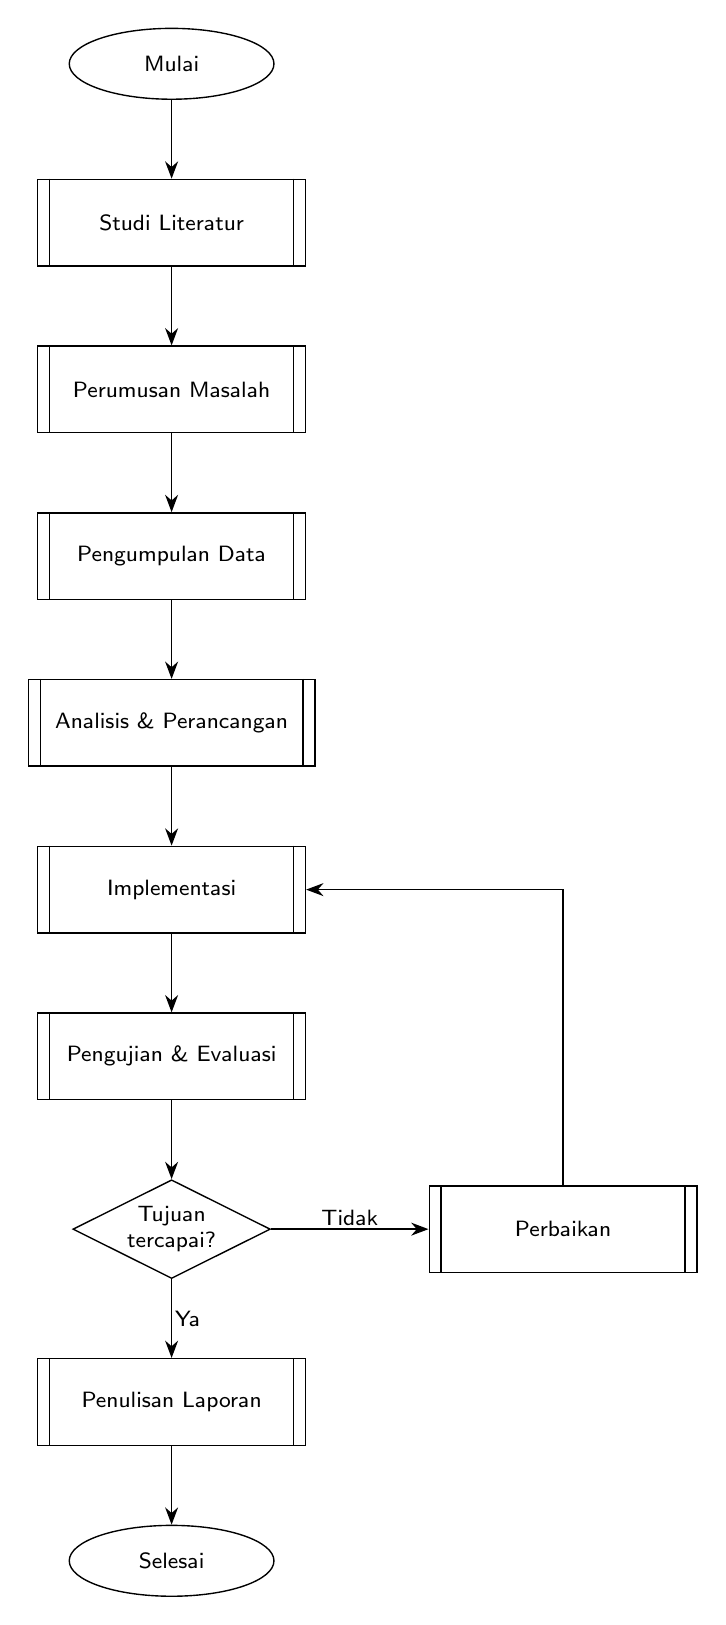
\begin{tikzpicture}[node distance=1cm]
  \node[term]    (mulai)   {Mulai};
  \node[proc]    (studi)   [below=of mulai]   {Studi Literatur};
  \node[proc]    (rumus)   [below=of studi]   {Perumusan Masalah};
  \node[proc]    (data)    [below=of rumus]   {Pengumpulan Data};
  \node[proc]    (analisis)[below=of data]    {Analisis \& Perancangan};
  \node[proc]    (impl)    [below=of analisis]{Implementasi};
  \node[proc]    (uji)     [below=of impl]    {Pengujian \& Evaluasi};
  \node[dec]     (valid)   [below=of uji]     {Tujuan \\ tercapai?};
  \node[proc]    (perbaiki)[right=2cm of valid]{Perbaikan};
  \node[proc]    (laporan) [below=of valid]   {Penulisan Laporan};
  \node[term]    (selesai) [below=of laporan] {Selesai};

  \draw[arr] (mulai)    -- (studi);
  \draw[arr] (studi)    -- (rumus);
  \draw[arr] (rumus)    -- (data);
  \draw[arr] (data)     -- (analisis);
  \draw[arr] (analisis) -- (impl);
  \draw[arr] (impl)     -- (uji);
  \draw[arr] (uji)      -- (valid);
  \draw[arr] (valid)    -- node[flbl,right]{Ya}  (laporan);
  \draw[arr] (valid)    -- node[flbl,above]{Tidak}(perbaiki);
  \draw[arr] (perbaiki) |- (impl);
  \draw[arr] (laporan)  -- (selesai);
\end{tikzpicture}
\end{document}
